\section{Theoretischer Hintergrund des Versuches}
\label{sec:Theorie}
In den folgenden Abschnitten werden die Grundlagen der Vakuumerzeugung beschrieben
sowie einige wichtige Begriffe definiert.

\subsection{Das Vakuum}
Der Begriff Vakuum ist definiert als der Zustand eines Gases, wenn der Druck
innerhalb eines Behälters geringer ist als außerhalb oder der Druck geringer
ist als $\SI{300}{\milli\bar}$, was der geringste auf der Erdoberfläche
vorkommende Druck ist.\\
Wenn Gase sich im Grenzfall einer verschwindenden Dichte befinden, ist das
ideale Gasgesetz \ref{eqn:idealesGas} eine gute Näherung:
\begin{equation}
 pV = N k_{B} T.
 \label{eqn:idealesGas}
\end{equation}
Hier bezeichnet $V$ das Volumen, $N$ die Teilchenanzahl, $k_{B}$ die
Boltzmann-Konstante, $T$ die Temperatur und $p$ den Druck.
Eine isotherme Zustandsänderung eines solchen idealen Gases kann beschrieben
werden durch das Boyle-Mariottesche Gesetz.
Es besagt, dass bei konstanter Temperatur und konstanter Stoffmenge der Druck direkt
proportional zum Volumen ist:
\begin{align}
  p & \propto \frac{1}{V} & \frac{p}{V} = \text{const}.
  \label{eqn:boylemariotte}
\end{align}
Der Druck ist definiert als eine senkrecht auf eine Fläche $A$ wirkende Kraft $F$:
\begin{equation}
  p = \frac{F}{A}.
  \label{eqn:druck}
\end{equation}
Der Partialdruck hingegen bezeichnet den Druck einer Komponente eines Gasgemischs.
Die Summe aller Partialdrücke ist daher bei idealen Gasen der Totaldruck. Dies
muss bei nicht idealen Gasen nicht notwendigerweise der Fall sein, da die Partialdrücke
sich allgemein gegenseitig stören können.\\
In SI-Einheiten wird der Druck in $\si{\pascal}$ angegeben. Der Zusammenhang zu dem
in Mitteleuropa gebräuchlicheren $\si{\bar}$ ist der Folgende:
\begin{equation}
 \SI{1}{\pascal} = \SI{0.01}{\milli\bar} = \SI{1}{\newton\per\square\meter}.
\end{equation}
Bei sehr geringen Drücken, wie z.B. im Weltall, ist die Angabe eines Drucks nicht
mehr praktikabel; stattdessen wird die Teilchenzahldichte verwendet. Diese gibt an,
wieviele Teilchen sich in einem gegebenen Raumbereich aufhalten.

\subsection{Wichtige Begriffe}
Im folgenden Abschnitt werden wichtige Begriffe im Zusammenhang mit Vakuumapparaturen
erklärt.

\subsubsection*{Die mittlere freie Weglänge}
Als mittlere freie Weglänge wird die Strecke bezeichnet, die ein Gasteilchen
auf geradem Weg im Mittel zwischen zwei Stößen zurücklegen kann.

\subsubsection*{Die verschiedenen Vakuums- und Strömungsarten}
Für eine Charakterisierung einer Strömung wird das Verhältnis aus mittlerer
freier Weglänge und dem Durchmesser des Strömungskanals verwendet. Hierfür wird die
Knudsen-Zahl definiert:
\begin{equation}
 Kn = \frac{\bar{l}}{d}.
\end{equation}
Hierbei bezeichnet $\bar{l}$ die mittlere freie Weglänge und $d$ den Durchmesser
des Strömungskanals. Je nach Größe der Knudsen-Zahl und die Art des Vakuums wird
zwischen Kontinuumsströmung, Knudsenströmung und Molekularer Strömung unterschieden:
\begin{figure}[H]
  \centering
  \includegraphics[scale=0.4]{pictures/strömungen.png}
  \label{fig:strömung}
  \caption{Abbildung der Strömungsarten abhängig von der Knudsen-Zahl \cite{pfeiffer}.}
\end{figure}
\noindent
Hierbei wird zwischen Grobvakuum, Feinvakuum und Hoch- bzw. Ultrahochvakuum unterschieden.
Grobvakuum meint dabei Drücke zwischen $\SI{300}{\milli\bar}$ und $\SI{1}{\milli\bar}$.
Hier finden hauptsächlich Stöße der Gasteilchen untereinander statt, was als Kontinuumsströmung
bezeichnet wird.
Innerhalb der Kontinuumsströmung wird weiter differenziert zwischen der laminaren
und der turbulenten Strömung. Die laminare Strömung wird auch als Schichtströmung
bezeichnet und besteht aus parallel angeordneten Schichten aus Gasteilchen. Durch
Erhöhung der Geschwindigkeit können diese Schichten aufgelöst werden. Dies führt
zu ungeordnet durcheinander laufenden Gasteilchen, was als turbulente Strömung
bezeichnet wird.\\
Innerhalb einer Vakuumapparatur kommt es nur beim schnellen Abpumpen von Atmosphärendruck
sowie bei schnellem Belüften zu turbulenter Strömung. Turbulente Strömung erfordert
höhere Saugvermögen der Vakuumpumpen, weshalb es günstig ist, turbulente Strömung durch
die richtige Dimensionierung der Strömungskanäle zu vermeiden. Um dies sicherzustellen,
reichen bei Grobvakua kleine Leiterdurchmesser, während bei Hoch- und Ultrahochvakua
größere Durchmesser nötig sind, um turbulente Strömung zu verhindern.\\
Das Feinvakuum ist definiert als Druckbereich von $\SI{1}{\milli\bar}$ und $\SI{1e-3}{\milli\bar}$.
Hier ist die mittlere freie Weglänge vergleichbar groß wie der Durchmesser des Strömungskanals,
weshalb die Gasteilchen hauptsächlich mit den Wänden des Gefäßes wechselwirken.
Die Strömung wird als Knudsen-Strömung bezeichnet.
Der Druckbereich von $\SI{1e-3}{\milli\bar}$ bis $\SI{1e-8}{\milli\bar}$ wird als Hochvakuum
bezeichnet. Bereiche darüber werden Ultrahochvakuum genannt. Hier ist die mittlere freie
Weglänge größer als der Durchmesser des Strömungskanals, weshalb hier kaum Wechselwirkung
der Gasteilchen untereinander stattfindet. Die sich ergebende Strömung heißt molekulare Strömung.

\subsubsection*{Die Absorption und Desorption}
Allgemein bezeichnet die Sorption einen Prozess, der zur Anreicherung eines Stoffes
innerhalb einer Phase oder an der Grenzfläche zwischen zwei Phasen führt.
Die Absorption bezeichnet hierbei die Anreicherung innerhalb einer Phase, während die
Anreicherung zwischen zwei Phasen als Adsoprtion bezeichnet wird. Handelt es sich nicht
um eine Aufnahme, sondern um eine Abnahme, wird von Desorption gesprochen.

\subsubsection*{Reale und virtuelle Lecks}
Als Lecks werden vakuummindernde Prozesse bezeichnet. Ein reales Leck ist eines,
das außerhalb der Vakuumanlage messbar ist, z.B. eine Undichtigkeit. Ein virtuelles
Leck hingegen ist eines, welches nicht außerhalb der Vakuumanlage erkennbar ist.
Beispiele hierfür sind Einschlüsse innerhalb der Anlage, welche nach einer Zeit an
die Materialoberfläche gelangen und austreten.
Eine Quelle von Lecks sind die obig erwähnten Desorptionen.

\subsubsection*{Das Saugvermögen einer Vakuumpumpe}
Um den obig erwähnten Lecks entgegenzuwirken, muss die Vakuumpumpe eine Saugleistung
besitzen, welche mindestens gleich der Leckrate ist. Das Saugvermögen ist definiert
als Volumenänderung pro Zeit:
\begin{equation}
 S = \frac{dV}{dt}.
\end{equation}
Die Bestimmung einer solchen Saugleistung kann z.B. durch die Aufnahme einer
Evakuierungskurve erfolgen. Dabei handelt es sich um die Druckänderung pro Zeit.

\subsection{Die Methoden der Vakuumerzeugung}

\subsubsection*{Kinetische Pumpen}
Das Funktionsprinzip einer kinetischen Pumpe ist die Beschleunigung der Teilchen in
die Pumprichtung. Eine solche Pumpe benötigt ein Vorvakuum, da bei einer zu hohen
Teilchendichte durch Kollisionen der Teilchen untereinander der Widerstand sehr hoch wird.
Durch ein Vorvakuum kann daher auch der Verschleiß einer solchen Pumpe reduziert werden.
Wenn das Vakuum hingegen schon recht gut ist, funktionieren kinetische Pumpen ebenfalls nicht
ideal, da die mittlere freie Weglänge ab einer gewissen Druckschwelle zu klein ist.
Die Teilchen ändern in diesem Fall ihre Bewegungsrichtung zu früh als dass sie in eine Richtung
beschleunigt werden könnten.

\subsubsection*{Gasfördernde Pumpen}
Nach \ref{eqn:boylemariotte} ist (bei konstanter Temperatur) der Druck
antiproportional zu dem Volumen. Dies wird von gasfördernden Pumpen ausgenutzt,
indem durch Komprimation und Ausdehnung Druckunterschiede erzeugt werden, welche
bei einem Ausgleichen der Drücke zu Teilchenströmen führen.

\subsubsection*{Gasbindende Vakuumpumpen}
Bei sehr hohen Vakua sind die obig erwähnten Pumpentypen weniger geeignet,
während die gasbindenden Vakuumpumpen hier sinnvoll eingesetzt werden können.
Durch Adsorption können bei einem bereits sehr hohen Vakuum immernoch effektiv
Gasteilchen gebunden werden. Dies ist weniger effektiv wenn die Teilchenanzahl sehr hoch ist,
in diesem Fall kann nur ein kleiner Teil der Gasteilchen gebunden werden.

\subsection{Die Drehschieberpumpe}
Drehschieberpumpen gehören zu den obig erwähnten gasfördernden Pumpen. Der schematische
Aufbau einer solchen Pumpe ist in Abbildung \ref{fig:drehschieber} gegeben.
\begin{figure}[H]
  \centering
  \caption{Der schematische Aufbau einer Drehschieberpumpe.}
  \label{fig:drehschieber}
  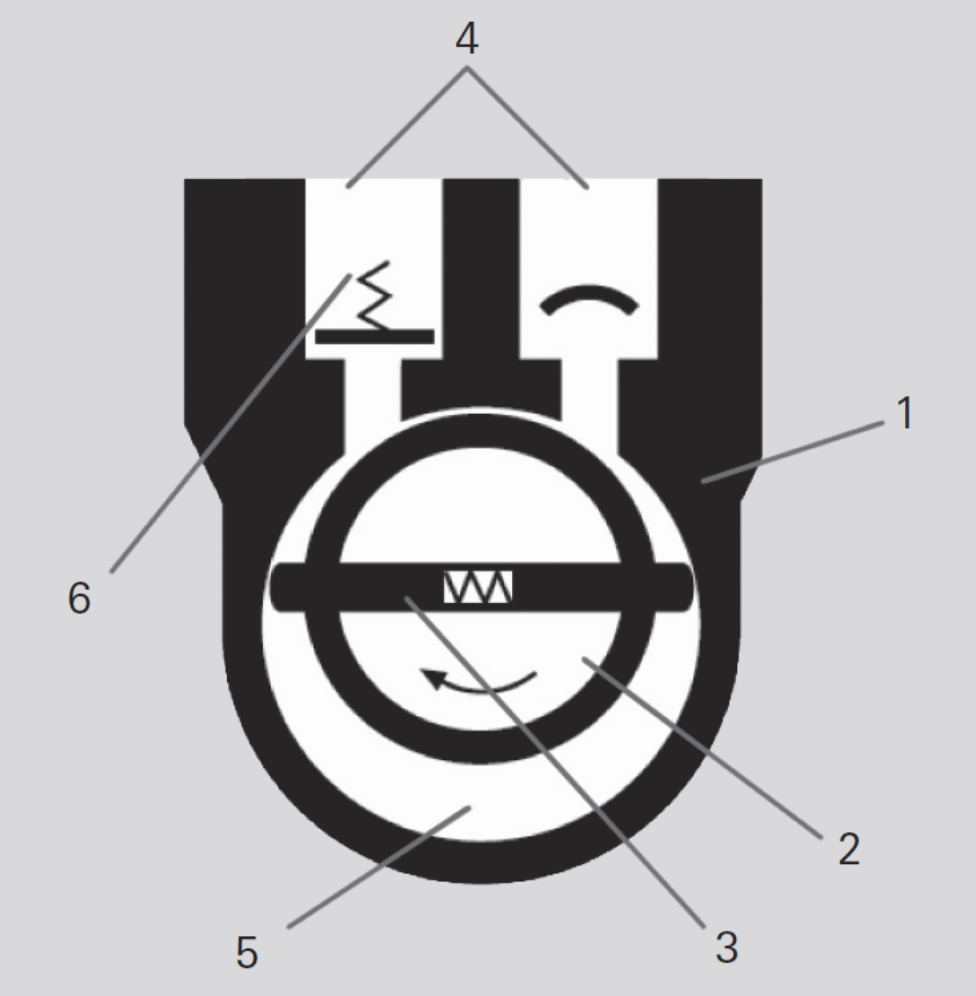
\includegraphics[scale=0.3]{pictures/drehschieber.png}
\end{figure}
\noindent
Der Arbeitsraum [5] einer Drehschieberpumpe wird durch die Schieber [3] des
Rotors [2] aufgeteilt und durch den Stator nach außen abgegrenzt.
Das Einlassventil [4] (rechte Seite) lässt im Betrieb Gas herinströmen.
Durch Drehen des Rotors [2] vergrößert sich das Volumen des Arbeitsraumes [5], bis der zweite Schieber
das Einlassventil abdeckt. Durch die exzentrische Rotation wird der Arbeitsbereich [5] durch die
weitere Drehung verkleinert, was eine Komprimation des Gases zur Folge hat. Das Auslassventil [4] (linke Seite)
öffnet sich bei genügend hoher Komprimation gegen den Atmosphärendruck, was ein Herausströmen des Gases zur
Folge hat. Durch die Ölschmierung des Auslassventils gerät bei jedem Öffnungsprozess eine
kleine Menge Öl in den Arbeitsraum, welches die Schieber gegen den Stator abdichtet. Daher haben
Drehschieberpumpen den Nachteil, dass durch Desorption von Teilchen aus dem verwendeten Schmieröl Lecks
entstehen. Es gibt ein- und
zweistufige Drehschieberpumpen, wobei die zweistufigen Pumpen geringere Drücke erreichen können.
Die in diesem Versuch verwendete zweistufige Drehschieberpumpe erreicht Drücke
von bis zu $p = \SI{2.1 e-2}{\milli\bar}$.

\subsection{Die Turbomolekularpumpe}
Die Turbomolekurlarpumpe gehört zu den kinetischen Pumpen. Eine Turbomolekularpumpe besteht
aus einem Rotor, welcher mit Schaufeln besetzt ist. Zwischen den Rotorschaufeln befinden sich
spiegelsymmetrische Statorschaufeln. Der Rotor dreht sich bei dem in diesem Versuch verwendeten
Exemplar mit bis zu $\SI{1350}{\hertz}$. Damit die Gasteilchen mit den Rotorschaufeln wechselwirken,
muss der Abstand der Rotorschaufeln ähnlich dimensioniert sein wie die mittlere freie Weglänge der
Gasteilchen. Zusätzlich sollte die Geschwindigkeit der Rotorblätter größer ist als die mittlere
Molekülgeschwindigkeit des Gases. Durch diese Wechselwirkung werden die Gasteilchen in die
gewünschte Pumprichtung beschleunigt. Der Rotor ist einseitig magnetgelagert, da
so eine Verwendung eines Öllagers vermieden werden kann.
